% !TeX spellcheck = pl_PL
\documentclass[12pt]{oska}

% Lista wszystkich języków stanowiących języki pozycji bibliograficznych użytych w pracy.
% (Zgodnie z zasadami tworzenia bibliografii każda pozycja powinna zostać utworzona zgodnie z zasadami języka, w którym dana publikacja została napisana.)
\usepackage[english,polish]{babel}

% Użyj polskiego łamania wyrazów (zamiast domyślnego angielskiego).
\usepackage{polski}
\usepackage[utf8]{inputenc}

% dodatkowe pakiety
\usepackage{mathtools}
\usepackage{amsfonts}
\usepackage{amsmath}
\usepackage{amsthm}
\usepackage[dvipsnames]{xcolor}
\usepackage{textcomp}

% obrazki
\usepackage{graphicx}
\usepackage{rotating}
\usepackage{caption}
\usepackage{float}

% --- < bibliografia > ---

\usepackage[
style=numeric,
sorting=none,
% Zastosuj styl wpisu bibliograficznego właściwy językowi publikacji.
language=autobib,
autolang=other,
% Zapisuj datę dostępu do strony WWW w formacie RRRR-MM-DD
%urldate=iso,
%seconds=true,
% Nie dodawaj numerów stron, na których występuje cytowanie
backref=false,
% Podawaj ISBN.
isbn=true,
% Nie podawaj URL-i, o ile nie jest to konieczne
url=false,
% Ustawienia związane z polskimi normami dla bibliografii
maxbibnames=6,
minbibnames=6,
% Jeżeli używamy Bibera:
backend=biber
]{biblatex}

\AtBeginBibliography{
\renewcommand\labelnamepunct{:\space}
\renewcommand\newunitpunct{\addcomma\space}
\renewcommand{\finentrypunct}{}

\renewcommand{\bibopenparen}{\addcomma\addspace}
\renewcommand{\bibcloseparen}{\addspace}
}

\usepackage{csquotes}
% Ponieważ `csquotes` nie posiada polskiego stylu, można skorzystać z mocno zbliżonego stylu chorwackiego.
\DeclareQuoteAlias{croatian}{polish}

% Przecinki do numerów
\usepackage{icomma}
% ------------------------

% --- < listingi > ---

% Użyj czcionki kroju Times.
\usepackage{newtxtext}

\usepackage{listings}
\lstloadlanguages{TeX}

\lstset{
	literate={ą}{{\k{a}}}1
           {ć}{{\'c}}1
           {ę}{{\k{e}}}1
           {ó}{{\'o}}1
           {ń}{{\'n}}1
           {ł}{{\l{}}}1
           {ś}{{\'s}}1
           {ź}{{\'z}}1
           {ż}{{\.z}}1
           {Ą}{{\k{A}}}1
           {Ć}{{\'C}}1
           {Ę}{{\k{E}}}1
           {Ó}{{\'O}}1
           {Ń}{{\'N}}1
           {Ł}{{\L{}}}1
           {Ś}{{\'S}}1
           {Ź}{{\'Z}}1
           {Ż}{{\.Z}}1,
	basicstyle=\footnotesize\ttfamily,
}

% ------------------------

\AtBeginDocument{
	\renewcommand{\tablename}{\textbf{Tabela}}
	\renewcommand{\figurename}{\textbf{Rysunek}}
}

% ------------------------
% --- < tabele > ---

\usepackage{array}
\usepackage{tabularx}
\usepackage{multirow}
\usepackage{booktabs}
\usepackage{makecell}
\usepackage[flushleft]{threeparttable}

% defines the X column to use m (\parbox[c]) instead of p (`parbox[t]`)
\newcolumntype{C}[1]{>{\hsize=#1\hsize\centering\arraybackslash}X}

\setlength{\cftsecnumwidth}{10mm}
\setcounter{secnumdepth}{4}
\brokenpenalty=10000\relax


%---------------------------------------------------------------------------

\titlePL{Wybrane aspekty modyfikacji obudowy zestawu głośnikowego}
\titleEN{Selected Aspects of Loudspeaker Cabinet Modifications}
\affiliation{Akademia Górniczo-Hutnicza im. S. Staszica w Krakowie}

%------------------------------------AUTORZY-----------------------

\namem{Michał}
\surnamem{Kmiecik}
\email{miszkoo@gmail.com} % adres do korespondencji -- zazwyczaj głównego autora

% Jeśli jesteś jedynym autorem pracy - pozostaw poniższe pola puste

\namei{Teresa}
\surnamei{Makuch}
\nameii{}
\surnameii{}

\nameiii{}
\surnameiii{}

\nameiiii{}
\surnameiiii{}

\nameiiiii{}
\surnameiiiii{}

%--------------------------STRESZCZENIE------------------------

\summaryPL{W procesie projektowania zestawu głośnikowego równie duże znaczenie, jak dobór przetworników, mają własności obudowy. Celem pracy było zbadanie wpływu różnych modyfikacji obudowy zestawu głośnikowego na jego parametry. W~związku z~tym wykonano pomiary impedancji elektrycznej, charakterystyk kierunkowości i~skuteczności zestawu, z~zastosowaniem różnych modyfikacji obudowy. Zarejestrowano także przebiegi drgań obudowy przy pomocy wibrometru laserowego. W~celu prowadzenia dalszych badań drogą symulacji, wykonano model komputerowy badanego zestawu przy użyciu metody elementów skończonych (MES).\\Podczas pomiarów zauważono znaczącą rozbieżność wyników z~danymi udostępnionymi przez producenta. W~związku z~tym przeprowadzono pomiary mające na celu weryfikację parametrów podanych w~karcie katalogowej.\\W~pracy zaprezentowano uzyskane wyniki, a~także spostrzeżenia związane z~wielokrotnym pomiarem i~zmiennością parametrów nowego przetwornika na skutek eksploatacji.}

\summaryEN{When designing a~loudspeaker, both the choice of transducers used and the cabinet characteristics are important. The authors’ aim was to investigate how different cabinet modifications influence the loudspeaker’s parameters. Therefore, loudspeakers' electric impedance, directivity characteristics and sensitivity were measured, covering various cabinet modifications. Vibrations of the cabinet were also recorded, using a laser vibrometer. In order to continue the research by simulation, a~computer model of the cabinet under inquiry was created using the finished elements method (FEM).\\During measurements, inconsistency between the obtained results and the producer’s data was discovered. Therefore, measurement aiming to verify parameters contained in datasheet was performed.\\The study presents obtained results and remarks on multiple measurement and fluctuation of a~new transducer’s parameters due to exploitation.}

%---------------------------------------------------------
% Nazwa pliku z bibliografią
%---------------------------------------------------------
\addbibresource{refs_OSKA.bib}
\graphicspath{{./}{obrazki/}}


\begin{document}

\maketitles

\section{Wstęp}

	\color{orange} Co w ogóle robimy, po co (może coś w~stylu, że chcieliśmy bardziej projektować, a~wyszło, że bardziej mierzyliśmy), plus trochę teorii (w~zależności, ile miejsca zajmie nam reszta...)
	\color{black}

\section{Badany zestaw głośnikowy}

	\color{orange} Napisać, że wysokotonowy to DE800, a niskotonowy to Beyma 10WR300. Opisać konstrukcję, zastosowane modyfikacje obudowy.
	\color{black}

	\begin{figure}[h!]
		\centering
% 		\includegraphics{}
		\caption{Fotografia badanego zestawu głośnikowego}
		\label{r:zdjecie}
	\end{figure}


\section{Metodyka pomiarów}

	W~celu możliwie dokładnego zbadania parametrów zestawu, ze szczególnym uwzględnieniem obudowy, zaplanowano szereg pomiarów: impedancji elektrycznej głośnika w~odgrodzie z~wyznaczeniem parametrów Thiele-Smalla, charakterystyki skuteczności, charakterystyk kierunkowości oraz pomiar drgań obudowy przy pomocy wibrometru laserowego -- metodykę wymienionych pomiarów opisano w~części~\ref{ss:metodyka}.
	
	Ze względu na zaobserwowane znaczące rozbieżności między wynikami uzyskanymi dla głośników niskotonowych, a~parametrami podanymi przez producenta w~karcie katalogowej, zdecydowano się na wykonanie dodatkowych pomiarów, uwzględniających zużycie głośnika; pomiary te opisano w~części~\ref{ss:dodatkowe}.
	
	Metodyka pomiarów opierała się na wytycznych zawartych w~normie EN 60268-5~\cite{norma}.

	\subsection{Przyjęta metodyka}\label{ss:metodyka}
	
		\subsubsection{Impedancja elektryczna i parametry Thiele-Smalla}
			
			Pomiary wykonano przy pomocy systemu Brüel\&Kjær PULSE, pozwalającego na pomiar charakterystyki impedancji oraz wyznaczenie na tej podstawie parametrów Thiele-Smalla.
			
			Do wyznaczenia tych parametrów wykorzystano metodę dodanej masy: wykonano pomiar impedancji głośnika, a~następnie do membrany przyklejono ciężarek o~masie $m=\,$\SI{10}{\gram} i~wykonano kolejny pomiar. Na podstawie porównania dwóch charakterystyk impedancji, za pomocą dedykowanego oprogramowania PULSE Thiele Small Parameters Calculation BZ-5604 wyznaczano parametry Thiele-Smalla~\cite{BK_pulse_TS}, opisane w~tabeli~\ref{t:TS_opis}.
			
			\begin{table}[h!]
				\centering
				\caption{Parametry Thiele-Smalla}
				\label{t:TS_opis}
				\begin{tabular}{|c|c|c|}
				\hline
					\textbf{Oznaczenie} & \textbf{Jednostka} & \textbf{Opis parametru}\\\hline\hline
					\multicolumn{3}{|c|}{Parametry wyznaczane z pojedynczego pomiaru} \\\hline\hline
					$F_s$ & Hz & Częstotliwość rezonansowa \\\hline
					$Z_{max}$ & \si{\ohm} & Impedancja w~rezonansie \\\hline
					$R_e$ & \si{\ohm} & Rezystancja dla napięcia stałego \\\hline
					$r0=\frac{Z_{max}}{R_e}$ & --- & Stosunek impedancji cewki do rezystancji \\\hline
					$S$ & \% & \makecell{Symetria rezonansu, wyznacznik wiarygodności\\obliczonych parametrów -- powinna wynosić najwyżej 3,5\%} \\\hline
					\hline
					$Q_{ms}$ & --- & Dobroć mechaniczna \\\hline
					$Q_{es}$ & --- & Dobroć elektryczna \\\hline
					$Q_{ts}=\frac{Q_{ms}\cdot Q_{es}}{Q_{ms}+Q_{es}}$ & --- & Dobroć całowita \\\hline
					\hline
					\multicolumn{3}{|c|}{Parametry wyznaczane z dwóch pomiarów (samej membrany i z dodaną masą)} \\\hline\hline
					$V_{as}$ & \si{\litre} & Równoważna objętość podatności głośnika \\\hline
					$M_{ms}$ & \si{\gram} & Masa mechaniczna membrany \\\hline
					$C_{ms}$ & \si[per-mode=symbol]{\metre\per\newton} & Podatność mechaniczna zawieszenia \\\hline
					$R_{ms}$ & \si[per-mode=symbol]{\metre\per\newton} & Rezystancja mechaniczna głośnika \\\hline
					\hline
					$M_{as}$ & \si[per-mode=symbol]{\kilo\gram\per\metre\tothe{4}} & Masa akustyczna membrany \\\hline
					$C_{as}$ & \si[per-mode=symbol]{\metre\tothe{5}\per\newton} & Podatność akustyczna zawieszenia \\\hline
					$R_{as}$ & \si[per-mode=symbol]{\newton\s\per\metre\tothe{5}} & Rezystancja akustyczna głośnika \\\hline
					\hline
					$\eta_0$ & \% & Sprawność głośnika \\\hline
				\end{tabular}

			\end{table}

			
			Sygnałem wykorzystanym w~pomiarze był sinus przestrajany w~zakresie \num{}--\num{}~\si{\Hz} co $1/24$~oktawy.
			
			Zmierzono impedancję głośnika niskotonowego w~odgrodzie, jednego głośnika w~obudowie oraz obu głośników w~obudowie.
			
		\subsubsection{Charakterystyka skuteczności}
			
			Do pomiarów wykorzystano analizator SVAN 912~E; głośnik pobudzano szumem różowym z~generatora o~wartości skutecznej \SI{1}{\watt}. Analizę prowadzono w~odległości \SI{2}{\metre} w~pasmach $1/3$-oktawowych w~zakresie \num{25}--\num{8000}~\si{\Hz}.
			
		\subsubsection{Charakterystyki kierunkowości}
			
			Wykonano dwie serie pomiarów, dla głośnika wysoko- i~niskotonowego. W~pierwszej serii zmierzono głośniki w~obudowie bez wypełnienia, w~drugiej -- wypełnione materiałem dźwiękochłonnym.
			
			Pomiar charakterystyki kierunkowości odbywał się w~komorze bezechowej przy użyciu stolika obrotowego, na którym umieszczony był zestaw głośnikowy. W~osi akustycznej mierzonego głośnika ustawiono mikrofon AE??; następnie głośnik obracano z~krokiem \SI{10}{\degree}, każdorazowo zatrzymując i~wykonując pomiar trwający \SI{3}{\s}. Sygnałem podawanym na głośnik był szum różowy, pomiar wykonano w~pasmach $1/6$~oktawy, w~zakresie \num{40}--\num{20000}~\si{\Hz}. \color{red} \textbf{Filtrowaliśmy???}\color{black}

			
		\subsubsection{Drgania obudowy}
			
			Pomiar drgań obudowy miał na celu sprawdzenie, w~jakim stopniu charakterystyka częstotliwościowa zestawu jest związana z~właściwościami obudowy. Badany zestaw głośnikowy umieszczono w~komorze bezechowej; w~wybranych punktach naklejono taśmę odblaskową, na którą padała wiązka lasera; wibrometr umieszczono w~odpowiedniej odległości, tak aby uniknąć przesterowania sygnału. Sygnałem pomiarowym był szum różowy, rejestrowano jednocześnie przebieg drgań wibrometrem oraz sygnał akustyczny mikrofonem umieszczonym blisko głośnika (rys.~\ref{r:zdjecie_wibro}). \color{red} \textbf{Czy na pewno tak, ew. podać odległości} \color{black}
			
			\begin{figure}[h!]
				\centering
				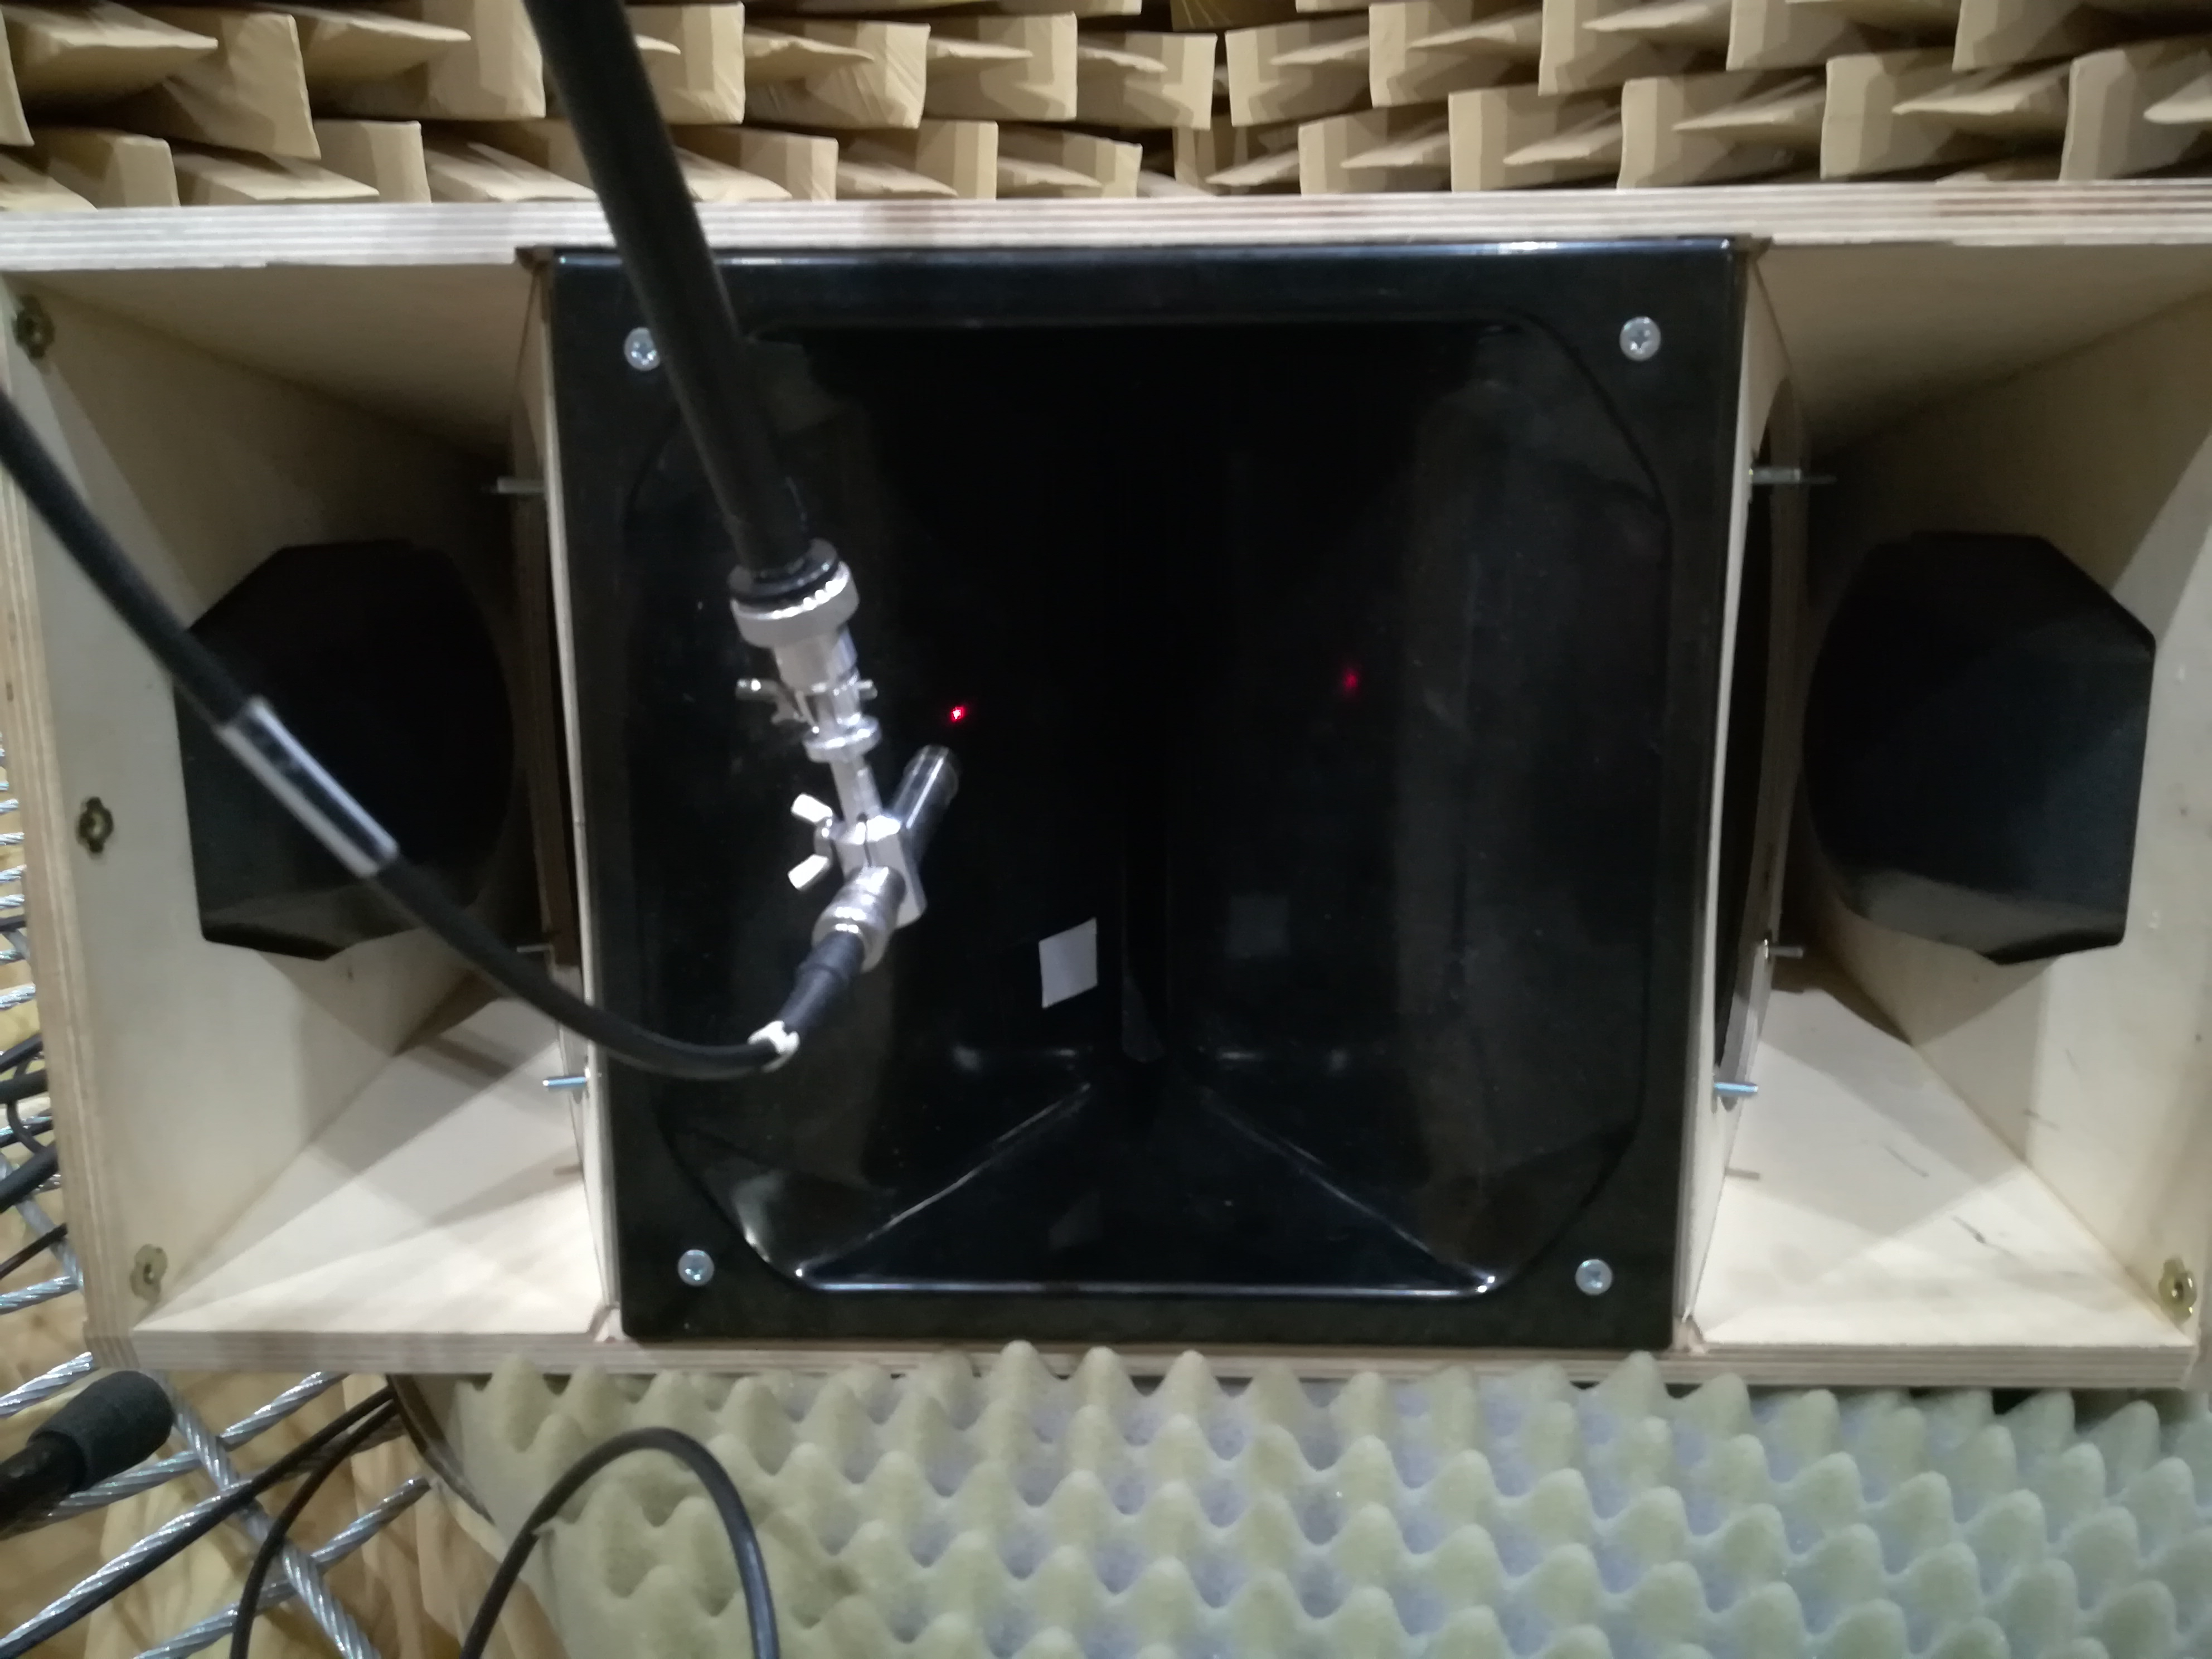
\includegraphics[width=\textwidth]{zdjecie_wibro.jpg}
				\caption{Fotografia wykonana podczas przygotowań do pomiaru z~użyciem wibrometru}
				\label{r:zdjecie_wibro}
			\end{figure}

	
	\subsection{Dodatkowe pomiary}\label{ss:dodatkowe}

\section{Modelowanie}

	\color{orange} Opis modelu w Comsolu, co modelowaliśmy, metody (?). To pisze Michał...
	\color{black}

\section{Analiza wyników}

	\subsection{Porównanie wyników pomiaru z~danymi producenta}
	
	\subsection{Porównanie wyników pomiaru, modelu i~parametrów teoretycznych}

\section{Podsumowanie}

\printbibliography

\end{document}
